\documentclass[aspectratio=169]{beamer}
\usetheme{Madrid}
\usecolortheme{default}
\usepackage[utf8]{inputenc}
\usepackage[T1]{fontenc}
\usepackage{booktabs}
\usepackage{tikz}
\usetikzlibrary{arrows.meta,positioning,shapes.geometric,fit}
\usepackage{hyperref}

\setbeamertemplate{navigation symbols}{}
\setbeamertemplate{footline}[frame number]
\setbeamerfont{title}{size=\Large,series=\bfseries}
\setbeamerfont{frametitle}{size=\large,series=\bfseries}

\title{Cloud File Service}
\subtitle{Transparent synchronization, passive replication, and sharing}
\author{J. Arévalo \and J. Gonzalez \and A. Baquedano \and L. Rodríguez}
\institute{Distributed Systems \\ Bachelor's Degree in Informatics Engineering}
\date{2026}

\begin{document}

\begin{frame}
  \titlepage
\end{frame}

\begin{frame}{Agenda}
  \tableofcontents
\end{frame}

\section{Problem and architecture}

\begin{frame}{Problem and objectives}
  \begin{itemize}
    \item A local folder must behave like a cloud folder.
    \item A server stores files and metadata; clients synchronize transparently.
    \item The server must survive the failure of its primary replica.
    \item Several users must share files and receive updates.
  \end{itemize}
  \vspace{0.4cm}
  \begin{block}{Scope}
    Proof of concept: three servers, two clients, manual/local deployment.
    The report explains what is implemented and what remains.
  \end{block}
\end{frame}

\begin{frame}{Architecture}
  \centering
  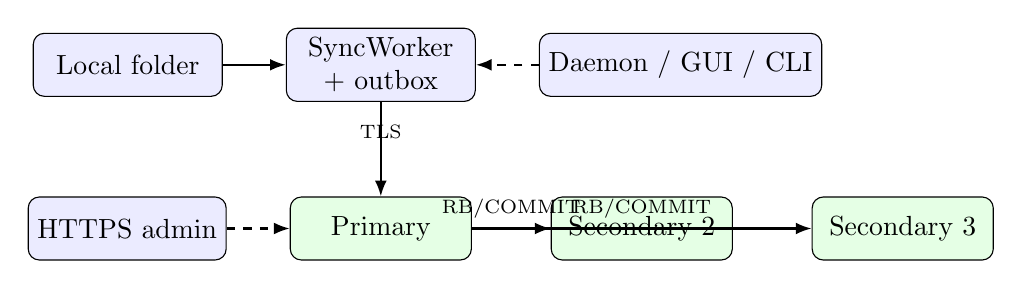
\begin{tikzpicture}[
    box/.style={draw, rounded corners, fill=blue!8, minimum width=2.4cm, minimum height=0.8cm, align=center},
    server/.style={draw, rounded corners, fill=green!10, minimum width=2.3cm, minimum height=0.8cm, align=center},
    arrow/.style={-{Latex[length=2mm]}, thick}
  ]
    \node[box] (fs) {Local folder};
    \node[box, right=0.8cm of fs] (sync) {SyncWorker\\+ outbox};
    \node[box, right=0.8cm of sync] (daemon) {Daemon / GUI / CLI};
    \node[server, below=1.2cm of sync] (p) {Primary};
    \node[server, right=1.0cm of p] (s2) {Secondary 2};
    \node[server, right=1.0cm of s2] (s3) {Secondary 3};
    \node[box, left=0.8cm of p] (admin) {HTTPS admin};
    \draw[arrow] (fs) -- (sync);
    \draw[arrow] (sync) -- node[above, font=\scriptsize]{TLS} (p);
    \draw[arrow] (p) -- node[above, font=\scriptsize]{RB/COMMIT} (s2);
    \draw[arrow] (p) -- node[above, font=\scriptsize]{RB/COMMIT} (s3);
    \draw[arrow, dashed] (daemon) -- (sync);
    \draw[arrow, dashed] (admin) -- (p);
  \end{tikzpicture}
  \vspace{0.3cm}
  \begin{itemize}
    \item Owned files at the root; shared files under \texttt{shared/<owner>/}.
    \item TLS is mandatory; replication uses mutual TLS.
  \end{itemize}
\end{frame}

\begin{frame}{Client transparency}
  \begin{itemize}
    \item \texttt{watchdog} observes creates, modifies, moves, and deletes.
    \item Events are coalesced and persisted in a SQLite outbox.
    \item Startup reconciliation compares the server manifest with the last
      known state and the local files.
    \item Uploads wait for size/mtime to stabilize.
    \item Downloads and remote deletes are written atomically.
  \end{itemize}
  \vspace{0.3cm}
  \begin{block}{Result}
    A client can be closed and restarted without losing pending changes.
  \end{block}
\end{frame}

\section{Replication and failure}

\begin{frame}{Passive replication}
  \begin{enumerate}
    \item The primary plans a deterministic operation: revision, hash,
      \texttt{mtime}, conflict name, and data.
    \item It sends \texttt{RB} to the secondaries and waits for ACK.
    \item With a 2/3 majority it appends a committed log entry.
    \item It applies the operation locally and sends \texttt{COMMIT}.
    \item Secondaries apply committed entries in order.
  \end{enumerate}
  \vspace{0.3cm}
  \begin{alertblock}{No quorum}
    The primary aborts the proposal, does not apply it, and returns \texttt{ER12}.
  \end{alertblock}
\end{frame}

\begin{frame}{Durable log and deterministic operations}
  \begin{columns}[T]
    \begin{column}{0.55\textwidth}
      \begin{itemize}
        \item Log entry: \texttt{(term, index, payload, committed)}.
        \item \texttt{commit\_index} and term are persisted.
        \item Operations are low-level writes, user updates, shares, and settings.
        \item Applying an operation never recalculates revisions or conflicts.
      \end{itemize}
    \end{column}
    \begin{column}{0.43\textwidth}
      \begin{block}{Why deterministic?}
        All replicas must produce the same bytes, hashes, and conflict names
        without relying on local clocks or local state.
      \end{block}
    \end{column}
  \end{columns}
\end{frame}

\begin{frame}{Election and fencing}
  \centering
  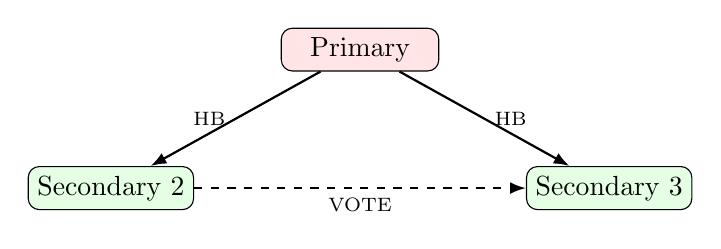
\begin{tikzpicture}[
    node distance=1.2cm,
    p/.style={draw, rounded corners, fill=red!10, minimum width=2cm},
    s/.style={draw, rounded corners, fill=green!10, minimum width=2cm},
    a/.style={-{Latex[length=2mm]}, thick}
  ]
    \node[p] (p) {Primary};
    \node[s, below left=1.2cm and 1.1cm of p] (s2) {Secondary 2};
    \node[s, below right=1.2cm and 1.1cm of p] (s3) {Secondary 3};
    \draw[a] (p) -- node[left,font=\scriptsize]{HB} (s2);
    \draw[a] (p) -- node[right,font=\scriptsize]{HB} (s3);
    \draw[a, dashed] (s2) -- node[below,font=\scriptsize]{VOTE} (s3);
  \end{tikzpicture}
  \vspace{0.3cm}
  \begin{itemize}
    \item Followers detect a missing heartbeat and start an election.
    \item Votes require a majority and a candidate log at least as recent.
    \item Higher terms fence the old primary.
    \item The leader steps down if it loses heartbeat quorum.
  \end{itemize}
\end{frame}

\begin{frame}{Failover and rejoin}
  \begin{enumerate}
    \item The old primary stops; a follower is elected.
    \item Clients ask \texttt{PRIM} and reconnect to the new primary.
    \item A restarted node becomes a follower.
    \item The leader detects its lagging \texttt{commit\_index}.
    \item The leader sends \texttt{SNAP}; the follower imports the snapshot and
      resets its log.
  \end{enumerate}
\end{frame}

\section{Sharing and interfaces}

\begin{frame}{Sharing and notifications}
  \begin{itemize}
    \item Owners grant \texttt{ro} or \texttt{rw} to another active user.
    \item Directory shares use prefix ACL checks; self-share is rejected.
    \item A stale write or delete creates a conflict copy.
    \item The primary's notification hub sends \texttt{UPDT} after commit.
    \item Active clients download/delete immediately; offline clients reconcile
      on restart.
  \end{itemize}
  \vspace{0.2cm}
  \begin{block}{Example}
    \texttt{shared/alice/docs/readme.txt} is editable by Bob with \texttt{rw}
    and restored remotely if Bob only has \texttt{ro}.
  \end{block}
\end{frame}

\begin{frame}{Desktop client and administration}
  \begin{columns}[T]
    \begin{column}{0.5\textwidth}
      \begin{block}{Desktop client}
        \begin{itemize}
          \item Tkinter GUI, tray, autostart.
          \item Background daemon owns the single worker.
          \item CLI controls the same daemon over local IPC.
        \end{itemize}
      \end{block}
    \end{column}
    \begin{column}{0.48\textwidth}
      \begin{block}{HTTPS admin}
        \begin{itemize}
          \item Users, shares, registration settings.
          \item Role, term, indexes, sessions.
          \item CSRF-protected sessions; secondary redirection.
          \item Demo-only step-down.
        \end{itemize}
      \end{block}
    \end{column}
  \end{columns}
\end{frame}

\section{Results and conclusions}

\begin{frame}{Results}
  \begin{table}
    \centering
    \begin{tabular}{ll}
      \toprule
      Check & Result \\
      \midrule
      Test suite & 174 tests passing \\
      Lint & \texttt{ruff check} clean \\
      Docs & strict MkDocs build \\
      Replicas & same state hash after mutations \\
      Failover & new primary well under 5 s \\
      Notifications & active client updated under 2 s \\
      Rejoin & old primary converges via snapshot \\
      Releases & server/client/GUI bundles build \\
      \bottomrule
    \end{tabular}
  \end{table}
\end{frame}

\begin{frame}{Limitations and pending work}
  \begin{itemize}
    \item Crash-stop model; no Byzantine faults or arbitrary partitions.
    \item No version history, tombstone GC, or chunked snapshots.
    \item Windows/Linux only; no macOS or signed installers.
    \item Admin panel lacks rate limiting and persistent audit.
    \item No email password reset or OS keyring integration.
    \item GUI/tray still needs final validation on a real desktop session.
  \end{itemize}
\end{frame}

\begin{frame}{Conclusions}
  \begin{itemize}
    \item The project implements the three course increments end to end.
    \item The main lesson is explicit failure handling: commit, fence, and
      rejoin are designed, not incidental.
    \item The system is intentionally a proof of concept, with documented
      boundaries and a clear path for production work.
  \end{itemize}
  \vspace{0.4cm}
  \centering
  \Large Questions?
\end{frame}

\end{document}
